% !TeX root = ../bbchallenge-paper.tex

\newpage



\begin{figure}[h!]
    \centering
    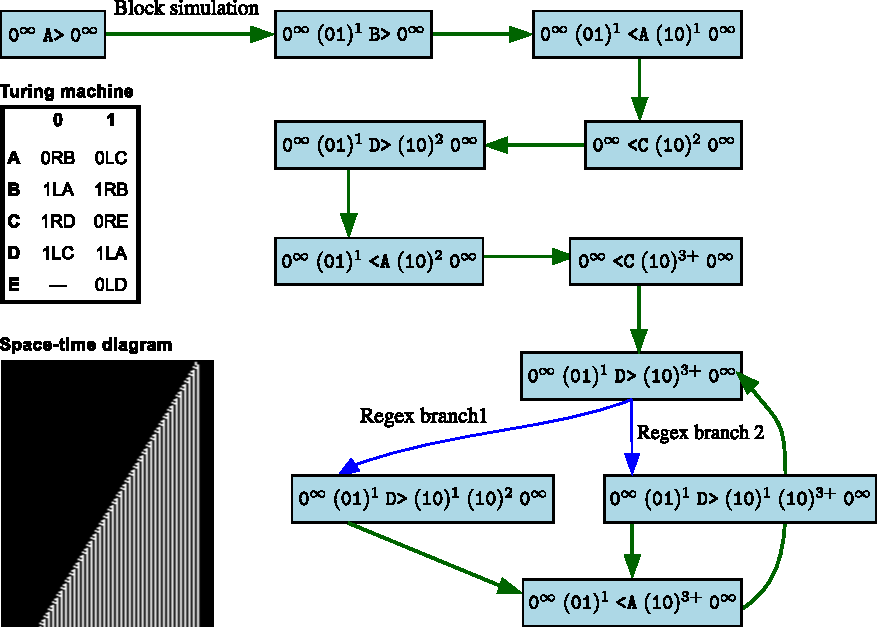
\includegraphics[scale=0.8]{figures/RepWL/RepWL_graph.pdf}
    \caption{{\small \textbf{RepWL graph.} Closed graph of regex configurations constructed by the Repeated Word List (RepWL) method (Section~\ref{sec:RepWL}) for machine \tm{0RB0LC_1LA1RB_1RD0RE_1LC1LA_---0LD} with block size $l=2$ and block repeat threshold $T=3$. Block simulation and regex branching steps (see Section~\ref{sec:RepWL}) are illustrated using respectively green and blue arrows. As illustrated by its 300-step space-time diagram, the machine is a simple Translated Cycler which can be easily handled by Section~\ref{alg:loops}, but this machine has the pedagogical advantage of having a very small graph. Because the graph is closed and contains not halting configuration, the machine does not halt, Theorem~\ref{th:repwl}.}}\label{fig:repWL}
\end{figure}

\begin{figure}[h!]
    \centering
    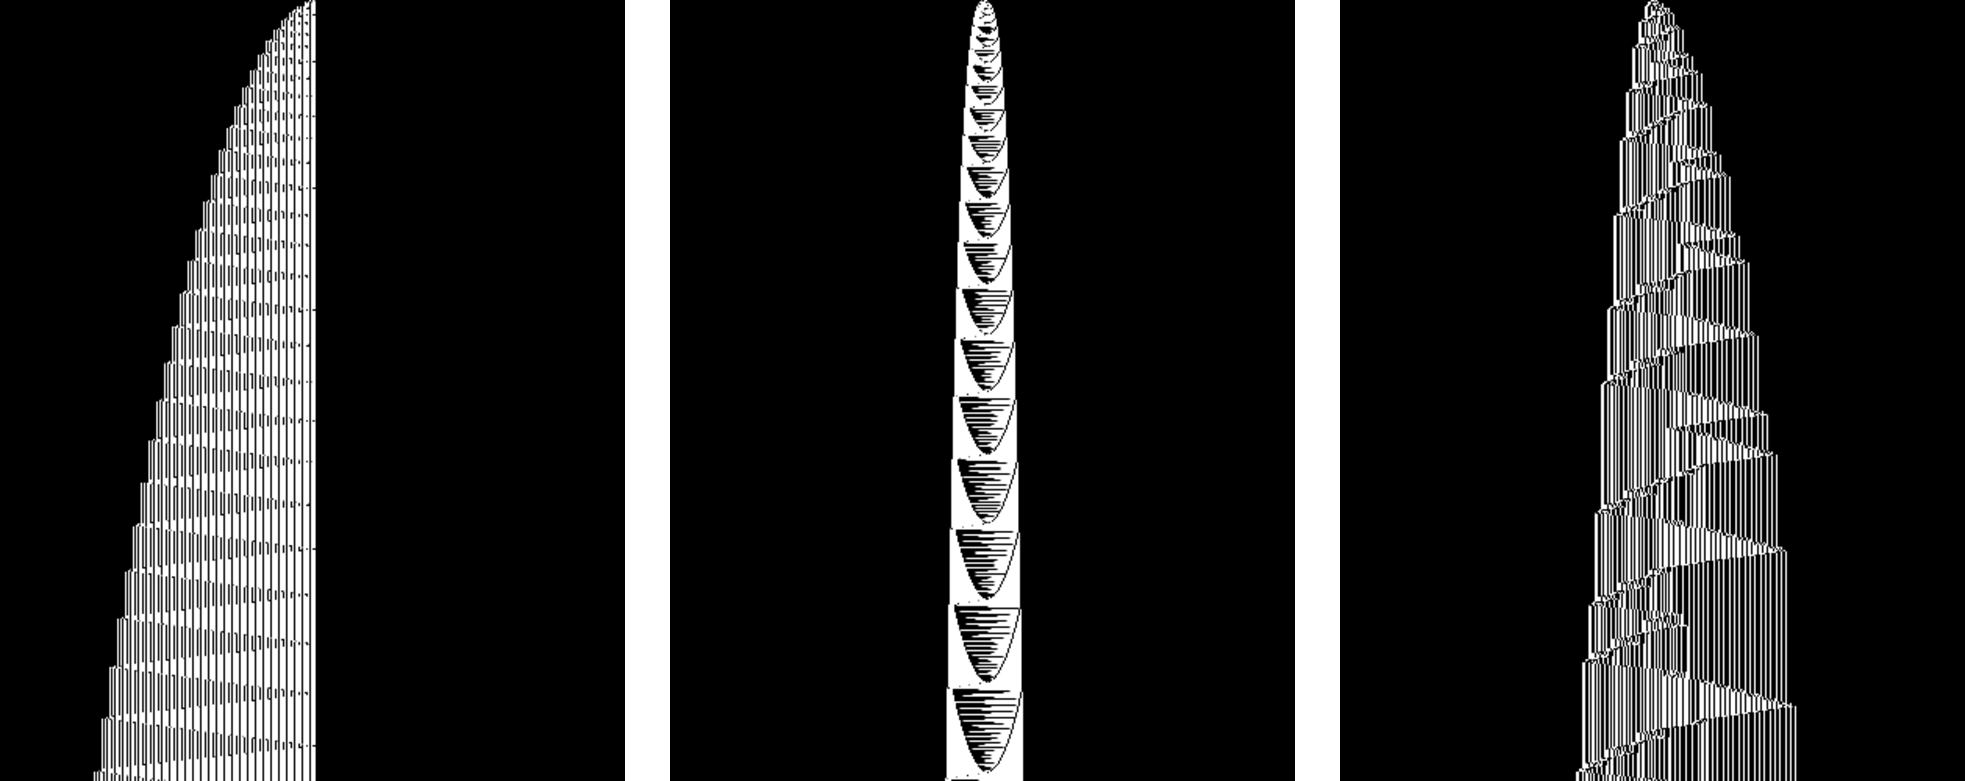
\includegraphics[scale=0.48]{figures/RepWL/RepWL_three_machines.pdf}
    \caption{10,000-step space-time diagrams of three 5-state machines decided by the Repeated Word List (RepWL) decider, Algorithm~\ref{alg:RepWL}. Left: {\small \tm{1RB0RD_0LC0LA_0LD1LC_1RA0LE_0RC---}}. Center: {\small \tm{1RB---_1LB1RC_1RA1RD_1LE0RD_0LB0LC}}. Right: {\small \tm{1RB---_0RC1RD_0LD1RC_1LE0RA_1RA0LE}}. The RepWL graphs of these machines respectively have 42 and $845$ and $143{,}181$ nodes, ranging the entire distribution of RepWL node counts for 5-state machines, see Section~\ref{sec:RepWL:results}. RepWL parameters $(l,T)$ for these machines are respectively: $(5,2)$, $(2,3)$, and, $(20,2)$.
    }\label{fig:repWLThree}
\end{figure}

% the machine's RepWL graph has 42 nodes (see Section~\ref{sec:RepWL}).
%, the machine's RepWL graph has $1{,}231$ nodes
% , the machine's RepWL graph has $143{,}181$ nodes
\subsection{Repeated Word List (RepWL)}\label{sec:RepWL}

\subsubsection{Algorithm}

The Repeated Word List (RepWL) technique, introduced by mxdys in \CoqBB, is based on the following simple idea: if a word (or \textit{block}) of length $l > 0$ appears consecutively on the tape more than $T > 0$ times (with $l, T \in \mathbb{N}$ fixed) then, we assume it may repeat an unbounded number of times in the future. In practice, it means we represent configurations as regular expressions. For instance, consider the following configuration:

$$ \texttt{0}^\infty \; \texttt{11100 A> 11110101010111111111} \; \texttt{0}^\infty$$

Using $l=2$ and $T = 3$, we represent it as:

$$ \texttt{0}^\infty \; (\texttt{01}) \; (\texttt{11}) \; (\texttt{00}) \; \texttt{A>} \; (\texttt{11})^2 \; (\texttt{01})^{3+} \; (\texttt{11})^{3+} \; \texttt{0}^\infty $$

Where blocks are constructed from the head outwards, and pumping symbols \szero out of $0^\infty$ if the number of symbols on either part of the tape is not a multiple of $l$. Any repetition of more than $T$ times the same word $w \in \{\szero,\sone\}^l$ is replaced by the regular expression $(w)^{T+}$ meaning that word $w$ is repeated at least $T$ times, hence the only exponents to ever be used in this representation are $\{1,2,\dots,T-1\}$ and $T+$. We call $T$ the block-repeat threshold. Note that here, we use \textit{directional head notation} for Turing machines, where the head lives in between cells and points either right or left. This framework is equivalent to the Turing machines setup used elsewhere in this work, see Section~\ref{sec:TMs}.

\paragraph{RepWL graph.} Using the rules explained below (\textit{block simulation} and \textit{regex branching}), {\sc decider-RepWL} (Algorithm~\ref{alg:RepWL}) simulates Turing machines directly on these regex configurations starting from the initial configuration (\ie $\texttt{0}^\infty \; \texttt{A>} \; \texttt{0}^\infty$), as to create a graph of such regex configurations to explore. If this graph is eventually closed (Algorithm~\ref{alg:RepWL}~l.\ref{alg:RepWL:closed}) and contains no halting configuration then we know that the machine will never halt (Theorem~\ref{th:repwl}) since we have constructed a set of configurations bigger than the one it will visit and that does not contain any halting transition. Because there is no guarantee the graph is closed, we also need an additional gas parameter (named $N$ in Algorithm~\ref{alg:RepWL}) indicating how many distinct nodes we're willing to visit at most. Figure~\ref{fig:repWL} gives the RepWL graph of a simple machine.

For simulating Turing machines on regex configurations we need to deal with two cases: (i) \textit{block simulation} when the head is facing a constant block (\ie block without a $+$), such as $\texttt{A>} \; (\texttt{11})^2$ and (ii) \textit{regex branching} when the head is facing a block with a $+$, \eg $\texttt{D>} \; (\texttt{01})^{3+}$.

\paragraph{Block simulation.} When the head is facing a constant block, such as in the above example $\texttt{A>} \; (\texttt{11})^2$ (or if the head is facing $0^\infty$, we add constant block $(\szero^l)^1$), we can proceed to \textit{block simulation}.
Block simulation consists of simulating the Turing machine until the head eventually leaves the block or until a maximum step limit is reached (parameter named $B$ in Algorithm~\ref{alg:RepWL}). Note that the TM may never leave the block if it enters an infinite cycle which is why we need the step limit -- one could alternatively implement cycle detection (Section~\ref{sec:loops}) in block simulation but it is not the route taken in \CoqBB. Depending upon which Turing machine is being simulated, block simulation from block simulation from $\texttt{A>} \; (\texttt{11})^2$ could produce, for instance, $(\texttt{00})^2 \; \texttt{B>}$ or $\texttt{<C} \; \texttt{10} \; \texttt{11} $ or enter a cycle and never leave the block. After block simulation, identical contiguous blocks are regrouped into powers, \eg $(\texttt{10})^1 \; (\texttt{10})^1 \; \texttt{B>}$ becomes $(\texttt{10})^2 \; \texttt{B>}$ and, assuming $T=3$, $(\texttt{10})^2\; (\texttt{10})^1\; \texttt{B>}$ would become $(\texttt{10})^{3+}\; \texttt{B>}$. In Figure~\ref{fig:repWL}, block simulation makes $\texttt{0}^\infty \; \texttt{A>} \; \texttt{0}^\infty$, which is first internally replaced with $\texttt{0}^\infty \; \texttt{A>} \; (\texttt{00})^1 \; \texttt{0}^\infty$, go to $\texttt{0}^\infty \; (\texttt{01})^1 \; \texttt{B>} \; \texttt{0}^\infty$.

\paragraph{Regex branching.} When the head is facing a block with a $^+$, for instance in Figure~\ref{fig:repWL} we have $\texttt{0}^\infty \; \texttt{01}^1 \; \texttt{D>} \; (\texttt{01})^{3+} \; \texttt{0}^\infty$, from we add two configurations to the set of configurations to visit next:
\begin{enumerate}
    \item \textbf{Regex branch 1.} We visit $\texttt{0}^\infty \; \texttt{01}^1 \; \texttt{D>} \; (\texttt{01})^1 \; (\texttt{01})^{2} \; \texttt{0}^\infty$.
    \item \textbf{Regex branch 2.} We visit $\texttt{0}^\infty \; \texttt{01}^1 \; \texttt{D>} \; (\texttt{01})^1 \; (\texttt{01})^{3+} \; \texttt{0}^\infty$.
\end{enumerate}
In both case, we've reduced to block simulation.

\begin{example}
    Figure~\ref{fig:repWL} gives the RepWL graph for machine \tm{0RB0LC_1LA1RB_1RD0RE_1LC1LA_---0LD}. This machine was chosen to illustrate the method on a small RepWL graph but the machine is a simple Translated Cycler that be decided using Section~\ref{sec:loops}.
\end{example}


\begin{theorem}[\CoqBB: \texttt{Lemma RepWL\_ES\_decider\_spec}]\label{th:repwl}
    Let $\mathcal{M}$ be a Turing machine $l\in \N^+$ the block-length parameter, $T \in \N^+$ the block-repeat threshold, $B \in \N$ the maximum number of steps allowed in block simulation and $N \in \N$ the maximum number of nodes we are willing to visit. Then, \textsc{decider-RepWL}($\mathcal{M}$, $l$, $T$, $B$, $N$) terminates and its result is correct -- see Algorithm~\ref{alg:RepWL}: if it returns \NONHALT then $\mathcal{M}$ does not halt from the all-$0$ tape.
\end{theorem}
\begin{proof}
    The algorithm terminates thanks to parameters $B$ and $N$. For a machine $\mathcal{M}$, the algorithm returns $\NONHALT$ (Algorithm~l.\ref{alg:RepWL:closed}) iff the RepWL graph of $\mathcal{M}$ contains less than $N$ nodes (\ie is closed), and contains no halting configuration (Algorithm~l.\ref{alg:RepWL:fail}). Since the set of configurations reached by the machine is a subset of the regular language consisting of the union of each node's regex configuration, which includes no halting configuration, we get that the machine cannot halt from the all-0 tape.
\end{proof}


\begin{algorithm}
    \caption{{\sc decider-RepWL}}\label{alg:RepWL}

    \begin{algorithmic}[1]
        \State{\textbf{Input:} A Turing machine $\mathcal{M}$, block-length parameter $l>0$, minimum size of nonconstant blocks $T>0$, maximum number of steps allowed in block simulation $B \in \mathbb{N}$, maximum number of distinct nodes we're willing to visit $N\in \mathbb{N}$.}
        \State{\textbf{Output:} \NONHALT if the decider detects that the machine doesn't halt and \UNKNOWN otherwise.}
        \State
        \State $\texttt{to\_visit} = [\texttt{A>}]$
        \State $V = \{\}$ \Comment{Visited regex configurations}
        \State \While{$|V| < N$ \textbf{and} $\texttt{to\_visit}.\textbf{len}() \neq 0$}
        \State $\texttt{regex\_config} = \texttt{to\_visit}.\textbf{pop}()$
        \State \If{$\texttt{regex\_config}$ is in $V$}
        \State \textbf{continue}
        \EndIf
        \State
        \State Insert $\texttt{regex\_config}$ in $V$
        \State \If{head is facing a constant block}
        \State $\texttt{new\_regex\_config} = \texttt{regex\_config}.\textbf{block\_simulation}(B)$
        \If{\texttt{new\_regex\_config} has halted (\ie undefined transition was met) \textbf{or} \\ $\quad \quad \quad \;\,\,\,$ limit $B$ was exceeded during block simulation}
        \State \Return \UNKNOWN \label{alg:RepWL:fail}
        \EndIf
        \State $\texttt{to\_visit}.\textbf{append}(\texttt{new\_regex\_config})$
        \Else \Comment{Head is facing a block with a $+$}
        \State $\texttt{regex\_config\_1}, \; \texttt{regex\_config\_2} = \texttt{regex\_config}.\textbf{regex\_branching}(M)$
        \State $\texttt{to\_visit}.\textbf{append}(\texttt{regex\_config\_1})$
        \State $\texttt{to\_visit}.\textbf{append}(\texttt{regex\_config\_2})$
        \EndIf
        \EndWhile

        \State \If{$|V| < N$}
        \State \Return{\NONHALT}\label{alg:RepWL:closed}
        \Else
        \State \Return{\UNKNOWN}
        \EndIf
    \end{algorithmic}
\end{algorithm}

\subsubsection{Implementations and results}\label{sec:RepWL:results}

% \begin{figure}
%     \centering
%     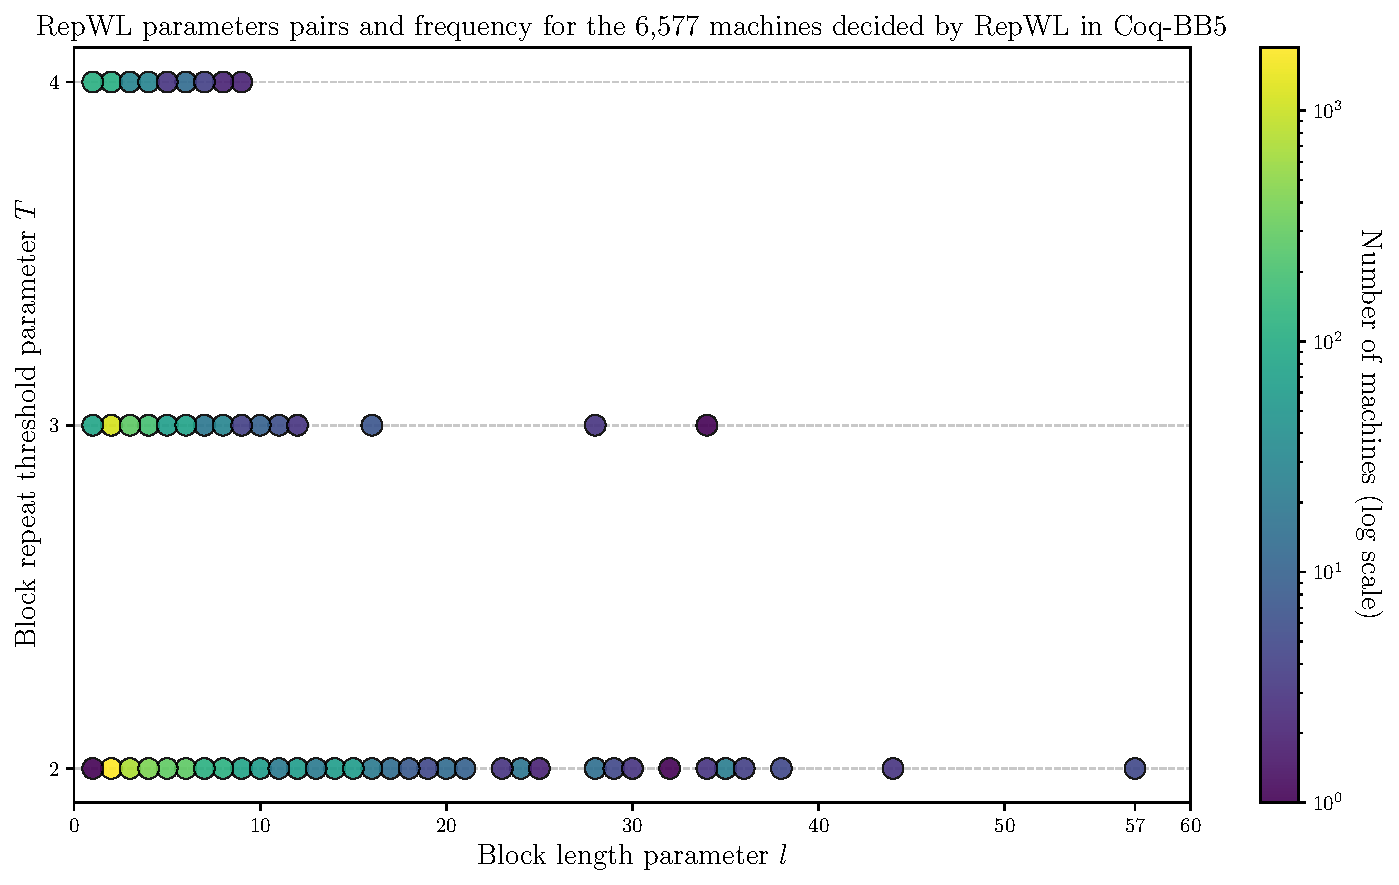
\includegraphics[scale=0.6]{figures/RepWL/repwl_parameters_pairs_log_scale.pdf}
%     \caption{Block length and repeat threshold parameters pairs $(l,T)$ and their frequency of use for the ${6,577}$ machines decided by RepWL in \CoqBB (see Table~\ref{tab:pipelineBB5}).}\label{fig:RepWLpairs}
% \end{figure}


% \begin{figure}
%     \centering
%     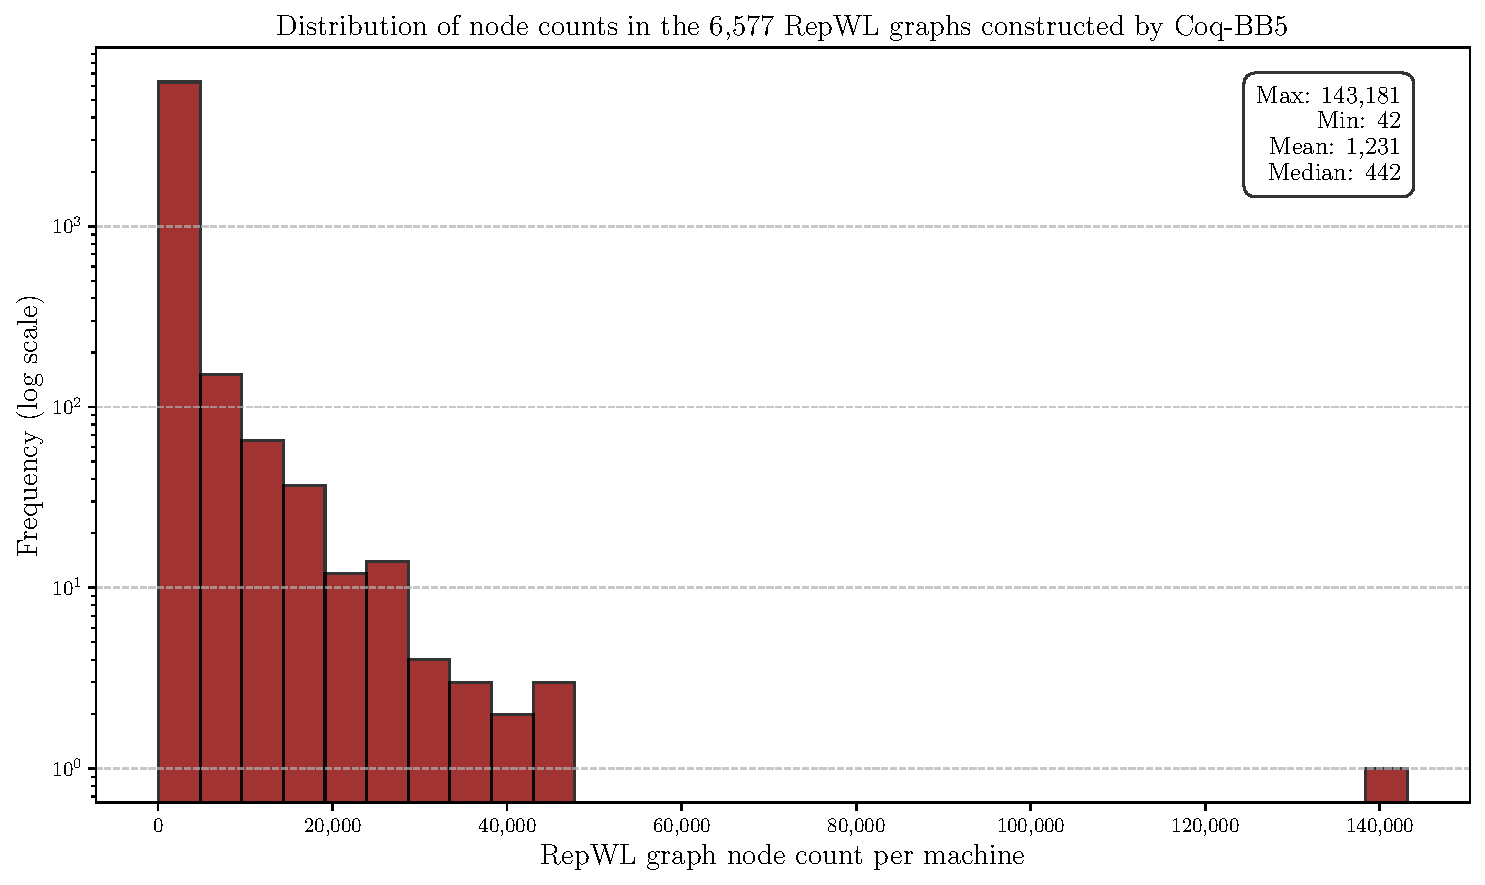
\includegraphics[scale=0.6]{figures/RepWL/repwl_node_counts_histogram.pdf}
%     \caption{distribution of node counts of the ${6,577}$ RepWL graphs constructed by \CoqBB.}\label{fig:RepWLhisto}
% \end{figure}


\CoqBB implements RepWL (Algorithm~\ref{alg:RepWL}), see function \texttt{RepWL\_ES\_decider}. Contrarily to previously presented deciders, RepWL is not applied in bulk using generic parameters. Instead, the ${6,577}$ machines it decides are hardcoded in the proof together with the specific $l$ and $T$ parameters that decide them -- see file \texttt{Decider\_RepWL\_Hardcoded\_Parameters.v}. Figure~\ref{fig:RepWLpairs} displays the $(l,T)$ pairs used for these ${6,577}$ machines. These parameters were found using a grid search in C++. For all these machines, maximum block simulation parameters and maximum number of graph nodes parameters are respectively set to 451 and ${150,001}$.

% Figure~\ref{fig:RepWLhisto} gives the distribution of node counts of the ${6,577}$ RepWL graphs constructed by \CoqBB. The average number of nodes is $1{,}231$ while minimum and maximum are respectively 42 and $143{,}181$. 
Figure~\ref{fig:repWLThree} gives space-time diagrams for machines with RepWL graphs with 42 (left), ${845}$ (center) and $143{,}181$ nodes. The machines on the left and on the right fit in the zoological category of \textit{Bouncers}, see Section~\ref{sec:zoo}. We developed a dedicated decider for solving Bouncers, but it was not used in \CoqBB \cite{bbchallenge_part1}.

In the $S(4)$ pipeline (Table~\ref{tab:pipelineBB4}), RepWL is only used to decide two machines using parameters $l=4$ and $T=3$. These 4-state machines are given in Figure~\ref{fig:RepWLBB4}, and they respectively have $3{,}130$ and $3{,}076$ nodes in their RepWL graph.

\begin{figure}
    \centering
    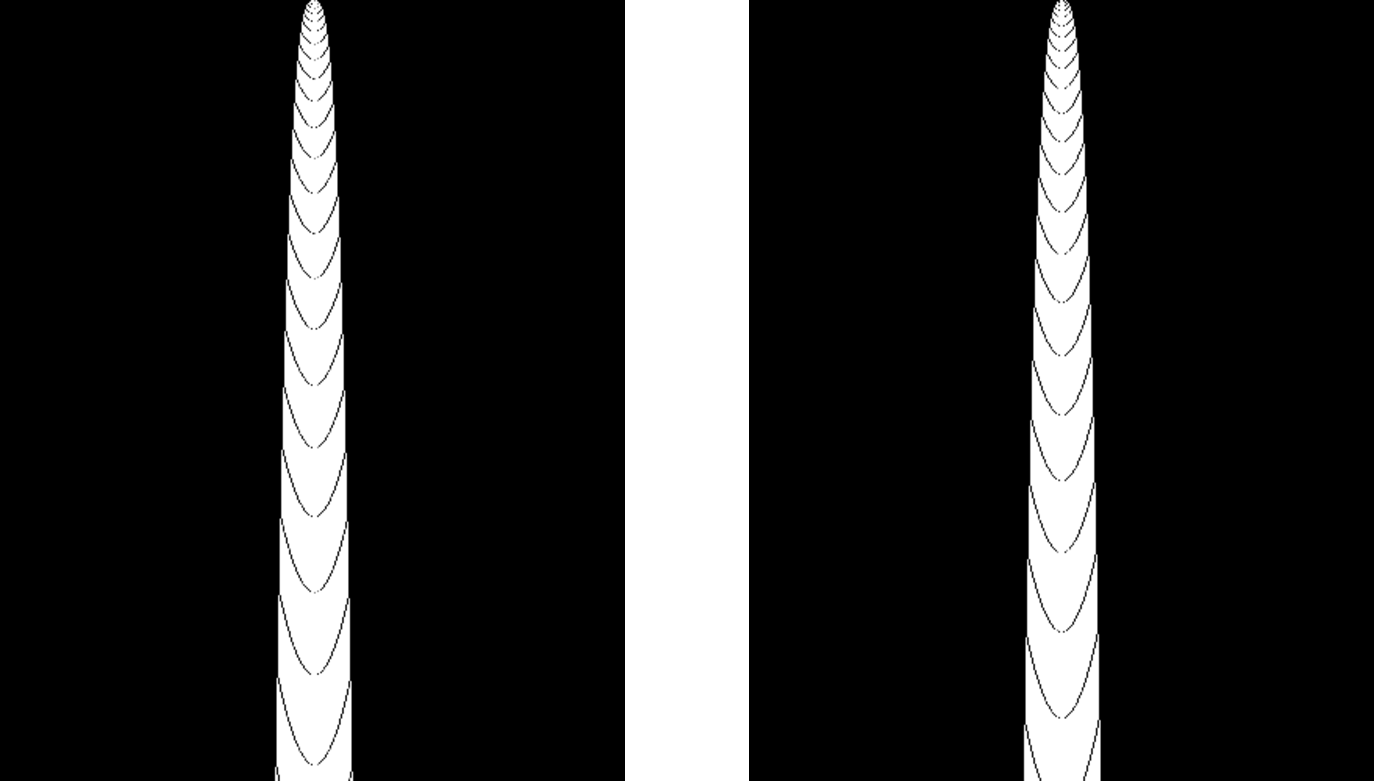
\includegraphics[scale=0.48]{figures/RepWL/RepWL_BB4_two_machines.pdf}
    \caption{10,000-step space-time diagrams of the two 4-state machines decided by the Repeated Word List (RepWL) decider in the $S(4)$ pipeline, Table~\ref{tab:pipelineBB4}. Left: {\small \tm{1RB1LA_1LA0RC_1LD1RC_---0LA}}. Right: {\small \tm{1RB0RB_1LC1RB_---0LD_1RA1LD}}. The RepWL graphs of these machines respectively have $3{,}130$ and $3{,}076$ nodes. Both machines are decided using $l=4$ and $T=3$.
    }\label{fig:RepWLBB4}
\end{figure}

\paragraph{Other implementations.} At the time of this writing, RepWL also has an Haskell and a Python implementation \cite{RepWL_haskell,RepWL_python}.